\documentclass[a4paper,12pt]{article}

\usepackage[utf8]{inputenc}
\usepackage[T1]{fontenc}
\usepackage{babel}
\usepackage{amsmath, amssymb, amsfonts}
\usepackage{graphicx}
\usepackage{hyperref}
\usepackage{geometry}
\usepackage{bookmark}
\geometry{a4paper, margin=1in}
\usepackage{luatexja}
\usepackage{luatexja-fontspec}
\setmainjfont{IPAexGothic}
\usepackage{tikz}
\usepackage{tikz-feynman}

\title{論文のタイトル}
\author{著者名}
\date{\today}

\begin{document}

\maketitle

\begin{abstract}
この論文の要約です。研究の概要、方法、結果、および結論を簡潔に示します。お願いします。
\end{abstract}

\section{Feynman図}
以下に、基本的なFeynman図の例を示します。

\begin{figure}[h]
    \centering
    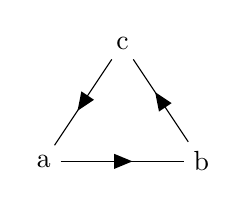
\begin{tikzpicture}
        \begin{feynman}
            \vertex (a) at (0,0) {a};
            \vertex (b) at (2,0) {b};
            \vertex (c) at (1,1.5) {c};

            \diagram* {
                (a) -- [fermion] (b) -- [fermion] (c) -- [fermion] (a),
                (b) -- [photon, out=45, in=135, loop, min distance=1.5cm] (b)
            };
        \end{feynman}
    \end{tikzpicture}
    \caption{基本的なFeynman図の例}
    \label{fig:feynman}
\end{figure}



\begin{table}[h]
  \centering
  \begin{tabular}{|c|c|c|}
      \hline
      名前 & 年齢 & 職業 \\
      \hline
      Alice & 24 & エンジニア \\
      \hline
      Bob & 27 & デザイナー \\
      \hline
      Charlie & 22 & データサイエンティスト \\
      \hline
  \end{tabular}
  \caption{サンプルの表}
  \label{tab:sample}
\end{table}


\section{Chern-Simons理論}
\begin{equation}
    S_{\mathrm{CS}} = \frac{k}{4\pi} \int_{\mathbb{R}^3} \epsilon^{\mu\nu\rho} \text{Tr} \left( A_\mu \partial_\nu A_\rho + \frac{2}{3} A_\mu A_\nu A_\rho \right) d^3x
\end{equation}
$ A_\mu = A_\mu^a T^a $ はSU(2)ゲージポテンシャル。
$ T^a $ はSU(2)の生成子であり、$ \text{Tr}(T^a T^b) = \frac{1}{2}\delta^{ab} $ を満たします。
$ \epsilon^{\mu\nu\rho} $ はレヴィ・チヴィタ記号です。
$ k $ は量子化されたレベル(整数値)です。

まず、トレースの中身を展開します:

\[
\text{Tr} \left( A_\mu \partial_\nu A_\rho + \frac{2}{3} A_\mu A_\nu A_\rho \right)
\]

これを成分ごとに書き下すと:

\[
\text{Tr} \left( A_\mu^a T^a \partial_\nu (A_\rho^b T^b) + \frac{2}{3} A_\mu^a T^a A_\nu^b T^b A_\rho^c T^c \right)
\]

生成子 $ T^a $ の性質 $ \text{Tr}(T^a T^b) = \frac{1}{2}\delta^{ab} $ を使うと:

\[
\text{Tr} \left( A_\mu^a T^a \partial_\nu (A_\rho^b T^b) \right) = A_\mu^a \partial_\nu A_\rho^b \text{Tr}(T^a T^b) = \frac{1}{2} A_\mu^a \partial_\nu A_\rho^b \delta^{ab} = \frac{1}{2} A_\mu^a \partial_\nu A_\rho^a
\]

同様に、三重項の部分も展開します:

\[
\text{Tr} \left( A_\mu^a T^a A_\nu^b T^b A_\rho^c T^c \right) = A_\mu^a A_\nu^b A_\rho^c \text{Tr}(T^a T^b T^c)
\]

ここで、SU(2)の生成子のトレースの性質を考慮すると、三重項のトレースは非ゼロの対称部分のみを考慮します。

これらをまとめると、Chern-Simons作用は次のように書き直せます:

\[
S_{\mathrm{CS}} = \frac{k}{4\pi} \int_{\mathbb{R}^3} \epsilon^{\mu\nu\rho} \left( \frac{1}{2} A_\mu^a \partial_\nu A_\rho^a + \frac{2}{3} f^{abc} A_\mu^a A_\nu^b A_\rho^c \right) d^3x
\]

ここで、$ f^{abc} $ はSU(2)の構造定数です。

このように、Chern-Simons作用の式を成分ごとに展開し、生成子の性質を利用して変形しました。

\section{方法}
このセクションでは、研究で使用された方法と手順を説明します。
今まで勉強した内容について詳しく説明します。具体的には、使用したデータセット、実験の手順、および分析方法について述べます。
\section{結果}
このセクションでは、研究の結果を示します。
\section{考察}
このセクションでは、結果を解釈し、その意味を議論します。
\begin{equation}
H = \sum_{i < j < k < l} J_{ijkl} \chi_i \chi_j \chi_k \chi_l
\end{equation}

\begin{figure}[h]
    \centering
    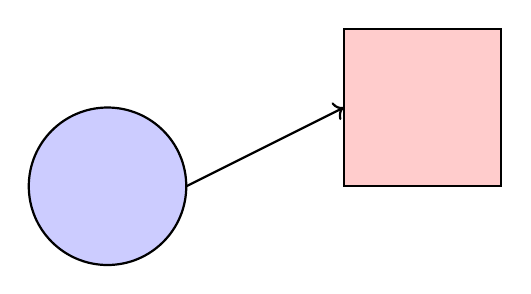
\begin{tikzpicture}
      % 円の描画
      \draw [thick, fill=blue!20] (0,0) circle [radius=1cm] node {円};
      
      % 四角形の描画
      \draw [thick, fill=red!20] (3,0) rectangle (5,2) node[midway] {四角形};
      
      % 矢印の描画
      \draw [->, thick] (1,0) -- (3,1);
    \end{tikzpicture}
    \caption{基本的な図形の例}
  \end{figure}
\section{結論}
このセクションでは、主な発見をまとめ、将来の研究の方向性を提案します。

\begin{thebibliography}{9}
\bibitem{example} 著者, \textit{書籍のタイトル}, 出版社, 年.
\end{thebibliography}

\end{document}